\documentclass[border=6pt]{standalone}
\usepackage{tikz}
\usepackage{pgfplots}
\pgfplotsset{compat=1.18}
\usetikzlibrary{arrows.meta,positioning,shapes.geometric,fit,backgrounds,calc,decorations.pathreplacing,patterns,pgfplots.groupplots}
\tikzset{
  blk/.style={rectangle, rounded corners=2pt, draw=black!70, thick, fill=blue!6,
              minimum height=8mm, minimum width=20mm, align=center, font=\small},
  io/.style={rectangle, rounded corners=6pt, draw=black!70, thick, fill=green!8,
             minimum height=8mm, align=center, font=\small},
  proc/.style={rectangle, draw=black!70, thick, fill=orange!10, minimum height=8mm,
               align=center, font=\small},
  dec/.style={diamond, aspect=2, draw=black!70, thick, fill=yellow!15, align=center, font=\footnotesize},
  warnbox/.style={rectangle, rounded corners=2pt, draw=red!60!black, thick, fill=red!7,
                  minimum height=8mm, align=center, font=\small},
  oklbox/.style={rectangle, rounded corners=2pt, draw=green!45!black, thick, fill=green!8,
                 minimum height=8mm, align=center, font=\small},
  ar/.style={-{Latex[length=2mm]}, thick},
  arl/.style={-{Latex[length=2mm]}, thick, dashed, draw=black!55},
  lbl/.style={font=\footnotesize\itshape, text=black!60},
}
\definecolor{good}{RGB}{34,139,34}
\definecolor{bad}{RGB}{178,34,34}
\definecolor{warn}{RGB}{218,165,32}
\definecolor{pesblue}{RGB}{0,45,98}
\definecolor{complete}{RGB}{30,125,79}
\definecolor{partial}{RGB}{176,106,0}
\definecolor{blocked}{RGB}{166,43,43}
\begin{document}
  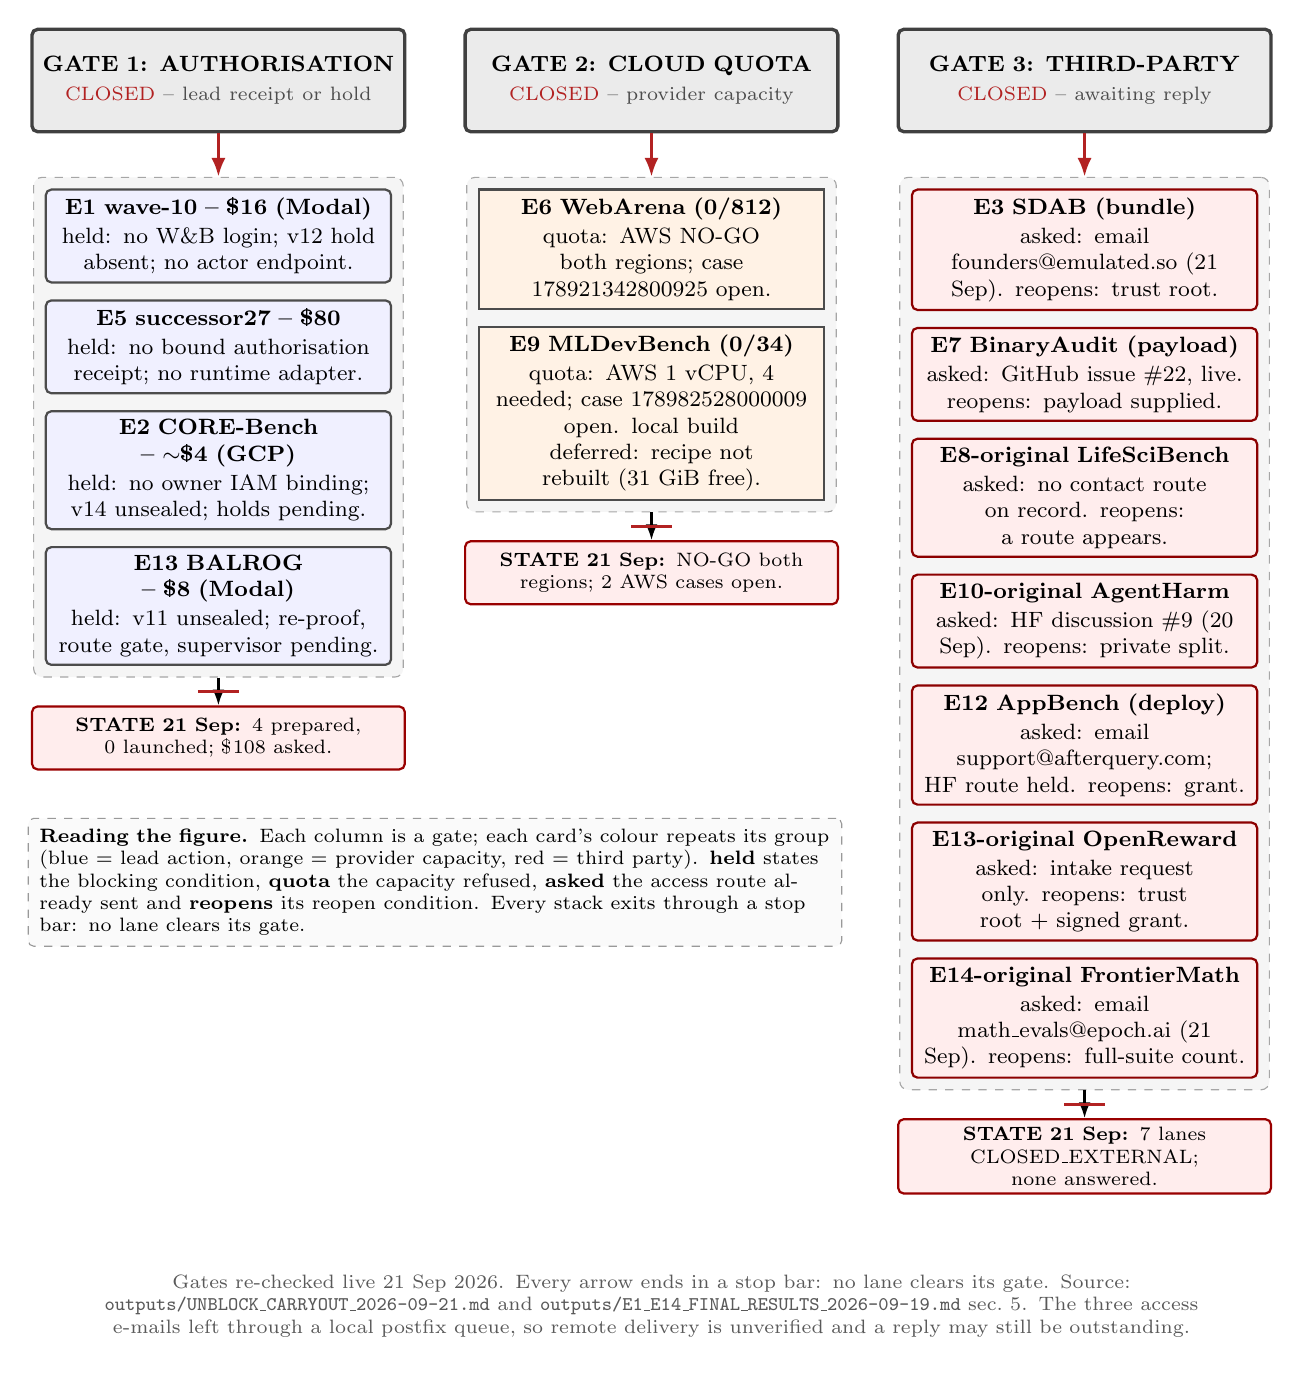
\begin{tikzpicture}[
      node distance=2mm,
      gate/.style={rectangle, rounded corners=2pt, draw=black!75, very thick,
                   fill=black!8, minimum height=13mm, text width=4.5cm,
                   align=center, font=\footnotesize, inner ysep=3pt},
      card/.style={blk, text width=4.15cm, font=\footnotesize, inner ysep=3pt},
      qcard/.style={proc, text width=4.15cm, font=\footnotesize, inner ysep=3pt},
      xcard/.style={warnbox, text width=4.15cm, font=\footnotesize, inner ysep=3pt,
                    draw=red!55!black, thick},
      state/.style={warnbox, text width=4.5cm, font=\scriptsize, inner ysep=3pt},
      panel/.style={fill=black!4, draw=black!35, dashed, rounded corners=3pt, inner sep=4pt},
      legendbox/.style={rectangle, rounded corners=2pt, draw=black!40, dashed,
                        fill=black!2, text width=10.5cm, align=left, font=\scriptsize,
                        inner sep=4pt},
    ]

    % ============================== Column 1: authorisation gate ==================
    \node[gate] (gA) at (0,0) {\textbf{GATE 1: AUTHORISATION}\\[1pt]
      {\normalfont\scriptsize\color{bad}CLOSED}\ {\normalfont\scriptsize\color{black!70}-- lead receipt or hold}};

    \node[card, below=7mm of gA] (a1)
      {\textbf{E1 wave-10 -- \$16 (Modal)}\\[1pt]
       held: no W\&B login; v12 hold absent; no actor endpoint.};
    \node[card, below=2mm of a1] (a2)
      {\textbf{E5 successor27 -- \$80}\\[1pt]
       held: no bound authorisation receipt; no runtime adapter.};
    \node[card, below=2mm of a2] (a3)
      {\textbf{E2 CORE-Bench -- $\sim$\$4 (GCP)}\\[1pt]
       held: no owner IAM binding; v14 unsealed; holds pending.};
    \node[card, below=2mm of a3] (a4)
      {\textbf{E13 BALROG -- \$8 (Modal)}\\[1pt]
       held: v11 unsealed; re-proof, route gate, supervisor pending.};

    \node[state, below=5mm of a4] (sA)
      {\textbf{STATE 21 Sep:} 4 \mbox{prepared}, 0 launched; \$108 asked.};

    \node[legendbox, below=6mm of sA, xshift=2.75cm, anchor=north, text width=10.05cm]
      {\textbf{Reading the figure.} Each column is a gate; each card's colour repeats its group
       (blue = lead action, orange = provider capacity, red = third party).
       \textbf{held} states the blocking condition, \textbf{quota} the capacity refused,
       \textbf{asked} the access route already sent and \textbf{reopens} its reopen condition.
       Every stack exits through a stop bar: no lane clears its gate.};

    % ============================== Column 2: quota gate ==========================
    \node[gate] (gB) at (5.5,0) {\textbf{GATE 2: CLOUD QUOTA}\\[1pt]
      {\normalfont\scriptsize\color{bad}CLOSED}\ {\normalfont\scriptsize\color{black!70}-- provider capacity}};

    \node[qcard, below=7mm of gB] (b1)
      {\textbf{E6 WebArena (0/812)}\\[1pt]
       quota: AWS NO-GO both regions; case 178921342800925 open.};
    \node[qcard, below=2mm of b1] (b2)
      {\textbf{E9 MLDevBench (0/34)}\\[1pt]
       quota: AWS 1 vCPU, 4 needed; case 178982528000009 open. local build
       \mbox{deferred}: recipe not \mbox{rebuilt} (31 GiB free).};

    \node[state, below=5mm of b2] (sB)
      {\textbf{STATE 21 Sep:} NO-GO both regions; 2 AWS cases open.};

    % ============================== Column 3: third-party gate ====================
    \node[gate] (gC) at (11.0,0) {\textbf{GATE 3: THIRD-PARTY}\\[1pt]
      {\normalfont\scriptsize\color{bad}CLOSED}\ {\normalfont\scriptsize\color{black!70}-- awaiting reply}};

    \node[xcard, below=7mm of gC] (c1)
      {\textbf{E3 SDAB (bundle)}\\[1pt]
       asked: email founders@emulated.so (21 Sep). reopens: trust root.};
    \node[xcard, below=2mm of c1] (c2)
      {\textbf{E7 BinaryAudit (payload)}\\[1pt]
       asked: GitHub issue \#22, live. reopens: payload supplied.};
    \node[xcard, below=2mm of c2] (c3)
      {\textbf{E8-original LifeSciBench}\\[1pt]
       asked: no contact route on record. \mbox{reopens}: a route appears.};
    \node[xcard, below=2mm of c3] (c4)
      {\textbf{E10-original AgentHarm}\\[1pt]
       asked: HF discussion \#9 (20 Sep). reopens: private split.};
    \node[xcard, below=2mm of c4] (c5)
      {\textbf{E12 AppBench (deploy)}\\[1pt]
       asked: email \mbox{support@afterquery.com}; HF route held. reopens: grant.};
    \node[xcard, below=2mm of c5] (c6)
      {\textbf{E13-original OpenReward}\\[1pt]
       asked: intake request only. reopens: trust root + signed grant.};
    \node[xcard, below=2mm of c6] (c7)
      {\textbf{E14-original \mbox{FrontierMath}}\\[1pt]
       asked: email \mbox{math\_evals@epoch.ai} (21 Sep). reopens: full-suite count.};

    \node[state, below=5mm of c7] (sC)
      {\textbf{STATE 21 Sep:} 7 lanes \mbox{CLOSED\_EXTERNAL}; none answered.};

    % ============================== panels + arrows ===============================
    \begin{scope}[on background layer]
      \node[panel, fit=(a1) (a4)] (pA) {};
      \node[panel, fit=(b1) (b2)] (pB) {};
      \node[panel, fit=(c1) (c7)] (pC) {};
    \end{scope}

    % gate -> held stack
    \draw[-{Latex[length=2.4mm]}, very thick, draw=bad] (gA.south) -- (pA.north);
    \draw[-{Latex[length=2.4mm]}, very thick, draw=bad] (gB.south) -- (pB.north);
    \draw[-{Latex[length=2.4mm]}, very thick, draw=bad] (gC.south) -- (pC.north);

    % held stack -> blocked exit (stop bar)
    \draw[ar] (pA.south) -- (sA.north);
    \coordinate (mA) at ($(pA.south)!0.5!(sA.north)$);
    \draw[very thick, draw=bad] ($(mA)+(-2.6mm,0)$) -- ($(mA)+(2.6mm,0)$);

    \draw[ar] (pB.south) -- (sB.north);
    \coordinate (mB) at ($(pB.south)!0.5!(sB.north)$);
    \draw[very thick, draw=bad] ($(mB)+(-2.6mm,0)$) -- ($(mB)+(2.6mm,0)$);

    \draw[ar] (pC.south) -- (sC.north);
    \coordinate (mC) at ($(pC.south)!0.5!(sC.north)$);
    \draw[very thick, draw=bad] ($(mC)+(-2.6mm,0)$) -- ($(mC)+(2.6mm,0)$);

    % ============================== provenance note ===============================
    \path (sC.south) node[below=9mm, xshift=-5.5cm, anchor=north, align=center,
        text width=15.6cm, font=\scriptsize, text=black!65]
      {Gates re-checked live 21 Sep 2026. Every arrow ends in a stop bar: no lane clears its gate.
       Source: \texttt{outputs/UNBLOCK\_CARRYOUT\_2026-09-21.md} and
       \texttt{outputs/E1\_E14\_FINAL\_RESULTS\_2026-09-19.md} sec.~5.
       The three access e-mails left through a local postfix queue, so remote delivery is
       unverified and a reply may still be outstanding.};

  \end{tikzpicture}
\end{document}
